\scanpage{118}
% archive sheet number: 117

$\otimes$-\uline{catégories}.

1) Définition. Catégorie \deleted{additiv} additive, avec bifoncteur
\[
(X,Y)\handwritten{\mapsto}X\otimes Y
\]
\deleted{et} un \deleted{objet} isomorphisme de bifoncteurs
\[
\handwritten{\phi}(X,Y,Z): (X\otimes Y)\otimes Z\handwritten{\xrightarrow{\sim}}X\otimes(Y\otimes Z)
\]
et un isomorphisme de commutativité
\[
\handwritten{\unsure{\mu|\psi}}(X,Y): X\otimes Y\handwritten{\xrightarrow{\sim}}Y\otimes X
\]
satisfaisant des axiomes

a) Axiome du pentagone pour $\handwritten{\phi}$ \deleted{(ne dépend pas de la structure additive)}

b) $\handwritten{\mu}(X,Y)\handwritten{\mu}(Y,X)=\mathrm{id}_{X\otimes X}$ \handwritten{;}

c) compatibilité entre $\handwritten{\phi}$ et $\handwritten{\mu}$ \handwritten{: axiome de l'hexagone}

d) existence d'un élément $1_C=\underline{1}$ , avec des isomorphismes fonctoriels
\[
u(X):\deleted{\unsure{x}}\quad\underline{1}\otimes X\handwritten{\simeq}X
\qquad\text{d'où}\quad
\inserted{v(X)=}\handwritten{\mu}(X,1)u(X): X\otimes1\handwritten{\simeq}X\ ,
\]
\figure{\handwritten{
\begin{tikzpicture}[x=1cm,y=1cm]
\draw (-.75,.05) .. controls (-.9,.7) and (.3,.3) .. (.5,.6);
\draw (-.6,.05) .. controls (-.4,-.45) and (.75,-.4) .. (.85,0) .. controls (.95,.6) and (1.5,.7) .. (1.85,.3);
\end{tikzpicture}}}
% The preceding figure records the transposition/enclosure strokes on the two factors; the typed order is retained in the display.
(donc par b on aura aussi $u(X)=v(X)\handwritten{\mu}(1,X)$)

avec la condition que pour $X=\underline{1}$, on trouve le même isomorphisme
\[
u(\underline{1})=v(\underline{1}) :\qquad \underline{1}\otimes\underline{1}\handwritten{\simeq}\underline{1}
\]
ce qui s'exprime aussi par la condition que $\handwritten{\mu}(\underline{1},\underline{1})=\mathrm{id}_{\underline{1}}$ \handwritten{;}

\margin{\handwritten{\figure{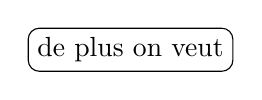
\begin{tikzpicture}
\node[draw,rounded corners,align=left] {de plus on veut};
\end{tikzpicture}}}}
\inserted{\handwritten{Compatibilité de $(\underline{1},u,v)$ avec $\unsure{\varphi|\phi}$, quand $X,Y$ \unsure{ou} $Z$ est \unsure{égal|ég.} à $1$, avec $\unsure{\psi|\mu}$ quand $X$ \unsure{ou} $Y$ est $=1$.}}

e) le foncteur $\otimes$ est biadditif.

\margin{\handwritten{\figure{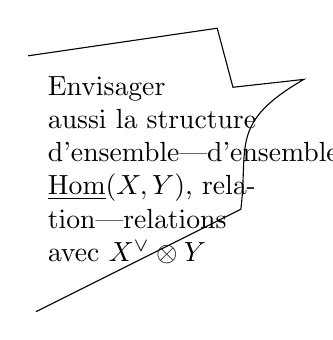
\begin{tikzpicture}[x=1cm,y=1cm]
\node[align=left,text width=2.7cm] at (0,0) {Envisager aussi la structure \unsure{d'ensemble|d'ensembles} $\underline{\mathrm{Hom}}(X,Y)$, \unsure{relation|relations} avec $X^\vee\otimes Y$};
\draw (-1.6,1.45) -- (.8,1.8) -- (1,1.05) -- (1.9,1.15) .. controls (.95,.6) and (1.2,.3) .. (1.1,-.5) -- (-1.5,-1.8);
\end{tikzpicture}}}}

NB a) \deleted{et d) sont}\inserted{est} indépendant\deleted{s} de la donnée de $\handwritten{\mu}$ , b) est indépendant de la donné de $\handwritten{\phi}$ , a)b)c)d) sont indépendant de fait que $C$ est additiv\deleted{\unsure{t}}e.

Soit $\underline{1}',u',\inserted{v'}$ comme $\underline{1},u,v$ , on va \deleted{définir canoniquement un}\inserted{\handwritten{voir qu'il existe un unique}} isomorphisme $w:\underline{1}\handwritten{\simeq}\underline{1}'$ , compatible en un sens évident avec $u,v$ et $u',v'$.

On choisit le composé
\diagram{\begin{tikzcd}[ampersand replacement=\&]
\underline{1} \arrow[r,"{\handwritten{\unsure{v'(1)|v(1)}}}"] \&
\underline{1}\otimes\underline{1}' \arrow[r,"{\handwritten{\unsure{u(\underline{1}')|\underline{1}\otimes u'}}}"] \&
\underline{1}'\deleted{\otimes\unsure{\underline{1}}} \arrow[r,phantom,"{\deleted{\longrightarrow}}" description] \& \deleted{\unsure{\underline{1}'}}
\end{tikzcd}}
. A vérifier les compatibilités annoncées (ne dépend pas de la donnée de $\handwritten{\phi}$, \inserted{ni $\handwritten{\mu}$,} mais de $u,v$ satisfaisant la compatibilité $\underline{u}(\underline{1})=v(\underline{1})$\deleted{\unsure{,}} et $u',v'$ kif-kif). C'est pourquoi il n'y\inserted{a} pas lieu de poser $\underline{1},u,v$ comme donnée, mais comme axiome d'existence.
